\subsubsection{nonnative-add}
\label{nonnative-add}

\begin{enumerate}
    \item target
        check the additional relation among three nonnative target objects.
    \item constraints-logic
        \begin{itemize}
            \item check equation for gadget,  a + b = c + modular * overflow
            \item check that "c lt modular"
        \end{itemize}
    \item nonnative-add process layout
        \begin{figure}[!ht]
            \centering
            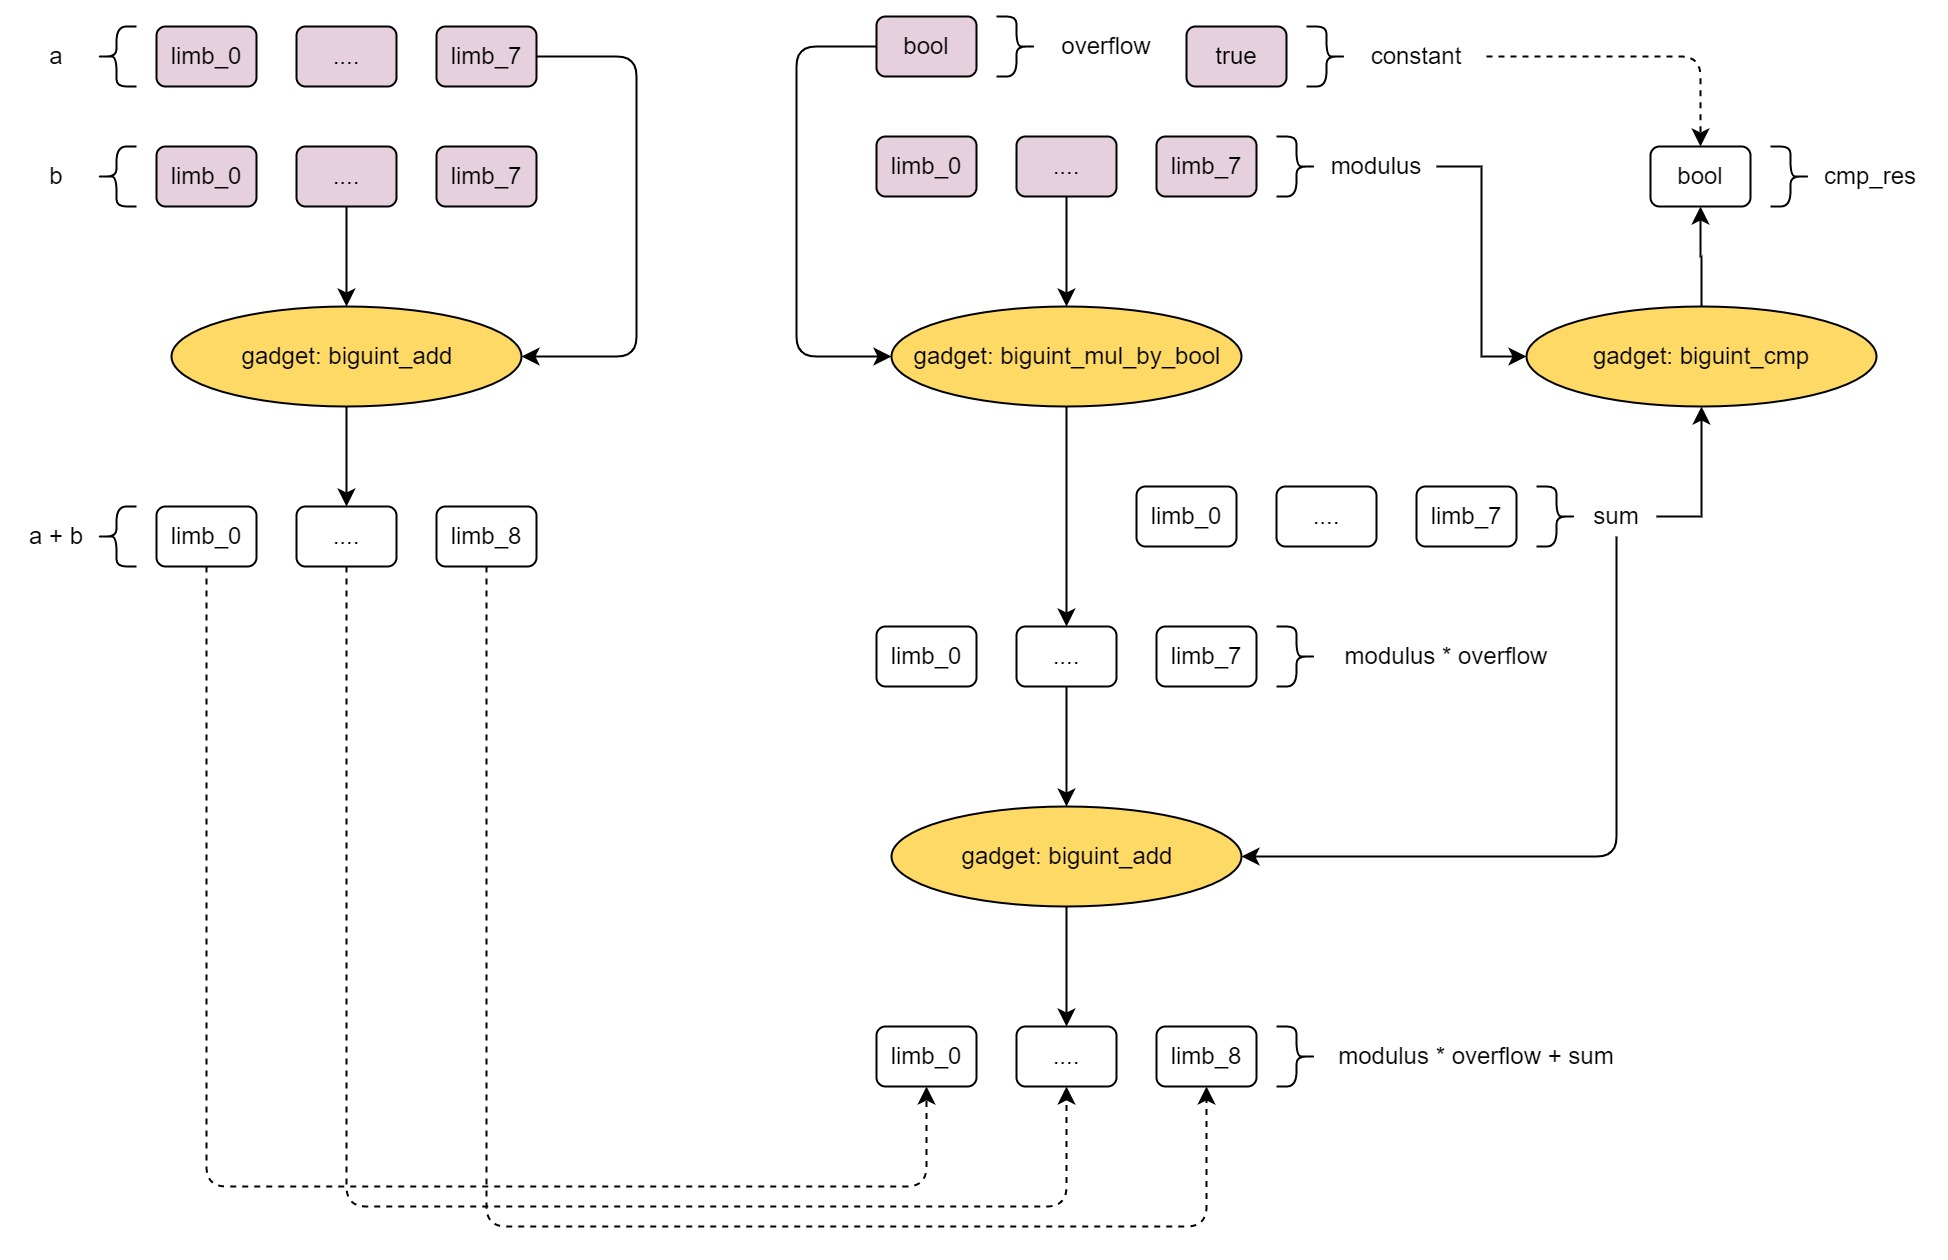
\includegraphics[width=0.8\textwidth]{nonnative-add-layout.jpg}
            \caption{nonnative-add layout}
            \label{fig:nonnative-add-layout}
        \end{figure}
    
    \item constraints-info and costs
        \begin{itemize}
            \item gadget biguint-add num: 2
            \item gadget biguint-mul-by-bool num: 1
            \item gadget biguint-cmp num: 1
            \item gate type num: 3(U32AddManyGate, ComparisonGate, ArithmeticGate)
            \item gate instance num: 23 = 3(U32AddManyGate) + 16(ComparisonGate) + 2(ArithmeticGate(1,0)) + 1(ArithmeticGate(1,-1)) + 1(ArithmeticGate(1,1))
            \item copy-constraints: 186 = 32 * 2{biguint-add} + 9{biguint-mul-by-bool} + 9 + (4 + 9) * 8{biguint-cmp} = 186
        \end{itemize}

    \item questions
        \begin{itemize}
            \item when set value to sum?
        \end{itemize}

\end{enumerate}